\documentclass{sig-alternate}
\usepackage{url}
\usepackage{enumitem}
\usepackage{cleveref}
\usepackage[titletoc,toc,title]{appendix}
\setdescription{noitemsep,topsep=0pt,parsep=0pt,partopsep=0pt}
 
\begin{document}
\conferenceinfo{1\textsuperscript{st} Web Audio Conference (WAC)}{, January 2015, Paris, France.
}
\title{Meyda: an audio feature extraction library for the Web Audio API}

\numberofauthors{3} 
\author{\hspace{-10 mm}Hugh Rawlinson\qquad Nevo Segal\qquad Jakub Fiala\vspace{2 mm}
\\\affaddr{Goldsmiths, University of London}\\
       \affaddr{New Cross}\\
       \affaddr{London}\\
       \affaddr{SE14 6NW}\\
       \email{mu202hr@gold.ac.uk}\quad
       \email{mu202ns@gold.ac.uk}\quad
       \email{mu201jf@gold.ac.uk}\quad
}

\maketitle
\begin{abstract}
There are many existing native libraries and frameworks for audio feature extraction used in multimedia information retrieval. Many are dependent on highly optimised low level code to cope with the high performance requirements of realtime audio analysis. In this paper, we present a new audio feature extractor library, Meyda\footnote{\url{github.com/hughrawlinson/meyda/tree/wac-release}}, for use with the JavaScript Web Audio API, and detail its benchmarking results. Meyda provides the first library for audio feature extraction in the web client, which will enable music information retrieval systems, complex visualisations and a wide variety of technologies and creative projects that previously were relegated to native software. The Meyda project, including source code and documentation is released under an MIT license.
\end{abstract}

\category{H.5.5}{Information Interfaces and Presentation}{Sound and Music Computing}[Systems]

\terms{Algorithms, Performance, Design}

\keywords{Audio Feature Extraction, Web Audio, Music Information Retrieval}\\

\vspace{10mm}
\section{Introduction}
The Meyda (from Hebrew - ``information'') library provides a research basis for further development of real-time client-side feature extraction in the context of the Web Audio API. It consists of an initial set of useful features for potential applications including multimedia information retrieval systems, complex audio visualisation, video game audio, and accessible demonstrations of related concepts for education across a variety of low-cost platforms. These initial features were chosen with influence from the set of features implemented in the YAAFE Audio Feature Extractor for Python, filtered by what was feasible in the context of the Web Audio API.

\section{Background}

Audio feature extraction is a very important field of research cultivated mainly in the Multimedia Information Retreival (MIR) community, whose main purpose is to ``provide new paradigms and methods for searching through the myriad variety of media all over the world''~\cite{lew2006}. Technologies developed within this community include algorithms for computer vision, media query-based search, media classification etc.

With the relatively recent emergence of the ``Web APIs'' including the Web Audio API~\cite{webaudiospec}, we are convinced that the Web is ultimately becoming a complete software platform capable of results comparable to hardware-dependent systems. It was with these facts in mind that we conceived the idea of enabling high-fidelity feature extraction in a Web environment, in particular the JavaScript-driven Web Audio API, whose processing features including the \mbox{ScriptProcessorNode}~\cite{webaudiospec} are crucial for accessing raw audio data and performing analysis.

The applications of such an implementation are numerous: speech recognition, for instance, utilises the \emph{Mel-frequency cepstral coefficients} feature~\cite{ganchev2005}. Despite the fact that there have been efforts to integrate speech recognition in web search interfaces~\cite{webspeechapispec}, these included an integrated low-level solution built in the browser architecture, not unlike other Web APIs. Other applications may use a server-side extraction library. Using a lightweight JavaScript-based implementation to obtain necessary feature data and apply recognition algorithms may prove a more flexible, customisable, and broadband-independent option for professional and academic use.

\section{Related Research}

Research in audio feature extraction has, despite being quite an established scientific field, found a great amount of new applications in the past three decades, in particular in the MIR community, with researchers beginning to adopt audio-based algorithms for not only sound media, but also corresponding video analysis, e.g. Rautiainen et al.~\cite{rautiainen2003}. Subsequently, after 2000, a substantial amount of audio feature extraction methods have been implemented as software products, even outside of academia. These are utilised in a variety of instances, including speech recognition~\cite{oshaughnessy2008}, music identification~\cite{wang2006}, multi-modal video summarisation~\cite{pan2004} etc.

Currently, there are already many native libraries for feature extraction on both Unix- and Windows-based systems. In particular, we were influenced by YAAFE~\cite{mathieu2010yaafe}, an open-source command line interface (CLI) for offline audio feature extraction~\cite{mathieu2010yaafe}, with most features adopted from the extensive list released as part of the CUIDADO project ~\cite{peeters2004large}. YAAFE is implemented in C++ and provides a Python wrapper for ease of use. We took cues as to which audio features to initially target for support from YAAFE's feature list. What is more, we used this library alongside the Java implementation of jAudio~\cite{mckay2005jaudio} during the testing process as a reference for validating extraction output. As for jAudio, it is an audio feature extraction library implemented in Java~\cite{mckay2005jaudio}. Accessible through a CLI or through a graphical user interface (GUI), it provides a number of statistical feature extractors as well as several semantic, MIR-oriented functions such as beat detection.

\section{Implementation Decisions}
\subsection{Design}
Perhaps the most significant design goal of Meyda was to provide simple integration into the existing Web Audio API node graph architecture. It integrates directly into the Web Audio API by accepting an \mbox{AudioContext}\cite{webaudiospec} and any node that implements the AudioNode interface as a source in the constructor of the object to be connected to Meyda's internal \mbox{ScriptProcessorNode}. We chose this architecture to provide the maximum ease of integration for users of the library. Meyda is intended as a terminating ``pseudo-node'' in the graph of nodes because it does not provide any transformations, rather, it takes data from the audio in the node graph and exposes it for usage in other contexts. As such, it does not implement the \mbox{AudioNode} interface because it should not be connected to a DestinationNode or any other further nodes.

There is significant continuing discussion as to how best to provide frequency domain data in the Web Audio API working group, in particular a split \cite{FFTinWebAudio} between providing a set of Fourier Transforms in the web audio, or waiting for the Web Array Math API\cite{WebArrayMathAPI} specification, which contains Fourier Transform functionality, to be formally submitted, reviewed, and implemented. Since the \mbox{AnalyserNode} containing an FFT implementation has a `black box'-style interface with few options and seemingly logarithmically scaled output, we used the existing open source \emph{jsfft} implementation of the Fast Fourier Transform (FFT) in JavaScript\cite{jsfft} which was released under an MIT License. Prior to the FFT, the time domain data is passed through a Hanning windowing function to improve the accuracy of the resulting frequency spectrum data.

Meyda was intended to provide a real-time Audio Feature Extraction API, and as such we placed great import on the optimisation of the feature extraction implementations. At a minimum, they were required to operate faster than real-time on what we decided were `reasonable' buffer sizes based on research into typical usage implementations of feature extraction on native platforms.

Concerning data output design, we found it important to provide some level of flexibility to the user, in order to enable both instantaneous (buffer-independent), and buffer-specific extraction. This is to ensure that, although the user can specify a custom extraction time or frequency, each `frame' of the incoming audio stream can be analysed specifically. Therefore we decided to implement two output systems:

\begin{itemize}
	\item \textbf{Immediate,} with a Meyda.get(features) method returning instantaneous data from the currently analysed real-time buffer.
	\item \textbf{Synchronized,} whereby a callback is specified in the Meyda constructor, executing desired code in sync with the internal \mbox{ScriptProcessorNode}. This is useful in instances where output is required for every buffer that is analysed by Meyda.
\end{itemize}

In order to simplify interaction with the API and to enable development of richer application structures, we decided to include a featureInfo object as a property of Meyda, carrying useful information about each of the implemented feature extractor functions, such as output type (``number'', ``array'', ``multipleArrays'') and, for some of the features, output range for automated visualisation.

\subsection{Implemented Features}
Our chosen implemented features fit into three distinct categories: perceptual features, time domain features, and spectral domain features. Time domain features are generally related to volume, while frequency statistics describe the shape of the spectrum and imply certain timbral characteristics. Perceptual features are features that are strongly correlated with human perception. As Meyda is a real-time audio analysis framework, the values are calculated on a per-frame basis, where the user of the library can specify the frame-length in the constructor of the Meyda instance. Meyda provides a callback to its enclosed \mbox{ScriptProcessorNode} to access each consecutive buffer of time and frequency domain that passes into the node.

The following is a list of features, and their definitions as implemented in Meyda\footnote{A more detailed description including implementation details, output information and sources is to be distributed as a text file in Meyda's production package}. These are identical in definition to their corresponding features in YAAFE, unless indicated otherwise.

\subsubsection{Time-Domain}

\begin{description}
       \item[RMS]\hfill \\
       The root mean square of the waveform calculated in the time domain to indicate its loudness. Corresponds to the `Energy' feature in YAAFE, adapted from Loy's \emph{Musimathics} \cite{loy2006}.
       \item[Energy]\hfill \\
       The infinite integral of the squared signal. According to Lathi \cite{lathi1998}.
       \item[Zero Crossing Rate]\hfill \\
       The number of times that the signal crosses the zero value in the buffer. Corresponds to ZCR in jAudio.
\end{description}

\subsubsection{Frequency-Domain}

\begin{description}
	   \item[Amplitude Ratio Spectrum (transformation)]\hfill \\
       Frequency domain amplitude spectrum, a transformation from the complex FFT.
       \item[Power Ratio Spectrum (transformation)]\hfill \\
       Frequency domain power spectrum, a transformation from the complex FFT.
       \item[Spectral Slope]\hfill \\
       A measure of how `inclined' the shape of the spectrum is. Calculated by performing linear regression on the amplitude spectrum.
       \item[Spectral Rolloff]\hfill \\
       The frequency below which is contained 99\% of the energy of the spectrum.
       \item[Spectral Flatness]\hfill \\
       The flatness of the spectrum as represented by the ratio between the geometric and arithmetic means. It is an indicator of the `noisiness' of a sound.
       \item[Spectral Centroid]\hfill \\
       An indicator of the brightness of a given spectrum, represents the spectral centre of gravity.
       \item[Spectral Spread]\hfill \\
       Indicates the `fullness' of the spectrum.
       \item[Spectral Skewness]\hfill \\
       Indicates whether or not the spectrum is skewed towards a particular range of values.
       \item[Spectral Kurtosis]\hfill \\
       The `pointedness' of a spectrum, can be used to indicate `pitchiness'.
       \item[Mel Frequency Cepstral Coefficients]\hfill \\
       A widely used metric for describing timbral characteristics based on the Mel scale. Implemented according to Huang  \cite{huang2001}, Davis \cite{davis1980}, Grierson \cite{grierson2010} and the \emph{librosa}\footnote{https://github.com/bmcfee/librosa} library
\end{description}
\subsubsection{Perceptual}

\begin{description}
       \item[Perceptual Loudness]\hfill \\
       The loudness of the spectrum as perceived by a human, using Bark bands. Outputs an object consisting of Specific Loudness (calculated for each Bark 		   band) and Total Loudness (a sum of the specific loudness coefficients).
       \item[Perceptual Spread]\hfill \\
       How `full' a human will perceive the sound to be.
       \item[Perceptual Sharpness]\hfill \\
       Perceived sharpness of the loudness Bark coefficients.
\end{description}

\subsubsection{Utility extractors}
\begin{itemize}
	   \item \textbf{Buffer}: a simple Float32Array of sample values
	   \item \textbf{Complex Spectrum:} a ComplexArray object carrying both real and imaginary parts of the FFT.
\end{itemize}

\subsection{Example implementation}
We have written a basic example of a webpage implementation using Meyda\footnote{http://hughrawlinson.github.io/meyda/examples/basic.html} to illustrate our design decisions with regards to how Meyda integrates with the Web Audio API. First, the Meyda library is included in the HTML source. An AudioContext is then instantiated, from which the source node for Meyda is created. The source node can be any of the Audio Nodes in the Web Audio API specification, or a node at the end of a chain in the context graph. At this point, the programmer instantiates a new Meyda object, passing the AudioContext, the source node, and the buffer size for analysis. Once Meyda's instantiation is complete, the user can then query the Meyda instance for the results of its feature extractors. This can be done as a one off query using Meyda's `get' function, or repeatedly by passing a callback as an additional argument to Meyda constructor, and calling `start', which will pass data back to the program for every buffer that is analysed.

\section{Testing and Benchmarking}
We ran some testing and benchmarking against Meyda on a mid-2010 Macbook Pro with a 2.53GHz Intel Core i5 processor with 4GB of RAM, using a Mozilla Firefox 32.0.3 browser. We feel that this machine represents a relatively standard modern hardware setup for desktop browsing.
\subsection{Testing}
To ensure accuracy of the implemented feature extractors, we tested the results of Meyda against those of YAAFE and jAudio. The latter was used initially: since jAudio analyses files on a frame average basis, we employed a rather tedious procedure to ensure the same buffer was being analysed:

\begin{enumerate}
	\item{Log time domain buffer and feature set from Meyda in the browser}
	\item{Save the time domain data to a PCM audio file (using a Puredata patch)}
	\item{Load the file into jAudio, set buffer size and feature extractors, and run extraction}
	\item{Compare the results}
\end{enumerate}

This approach was partially useful for validating the output of some features. However, we found the above workflow to be rather costly in terms of time. Therefore, we decided to rely on YAAFE, which has a more similar set of extractors and outputs frame-by-frame results. The procedure was thus largely simplified, using a 10-second recording of pure white noise as the analysis input:

\begin{enumerate}
	\item{Log feature set from Meyda in the browser}
	\item{Run YAAFE extraction with the same buffer size from the command line}
    \item{Compare the results from YAAFE CSV and Meyda's console output}
\end{enumerate}

\begin{figure}[ht!]
\centering
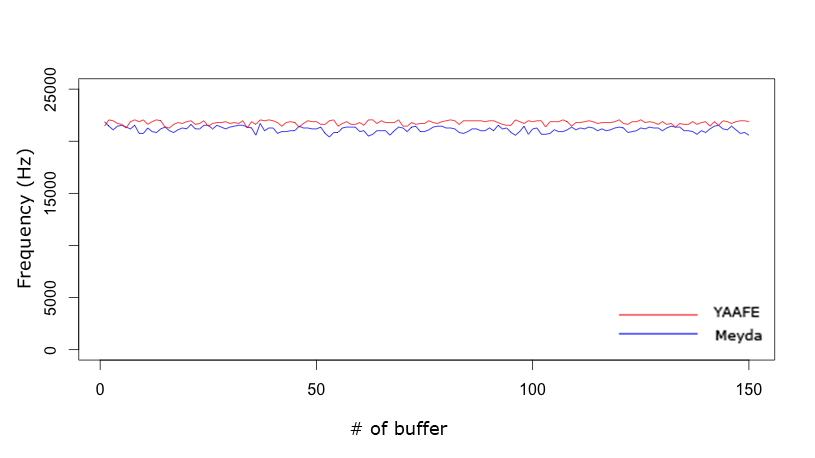
\includegraphics[width=70mm]{SR.png}
\caption{Spectral Rolloff comparison}
\label{fig:rolloff}
\end{figure}

\begin{figure}[ht!]
\centering
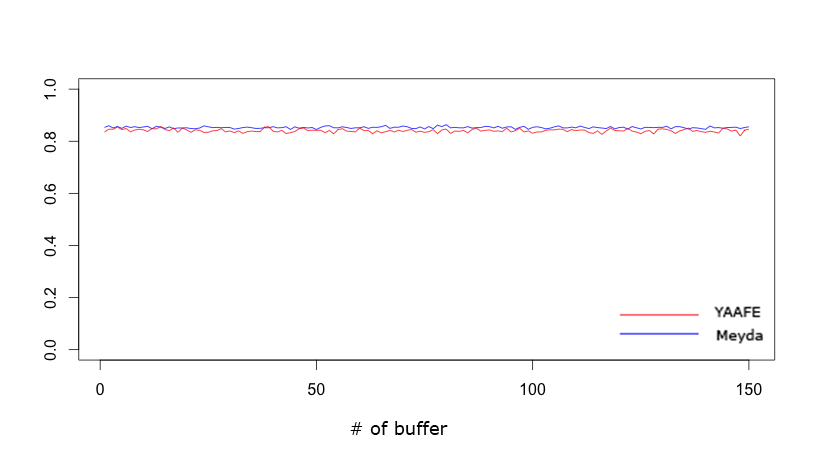
\includegraphics[width=70mm]{PSP.png}
\caption{Perceptual Spread comparison}
\label{fig:spread}
\end{figure}

\begin{figure}[ht!]
\centering
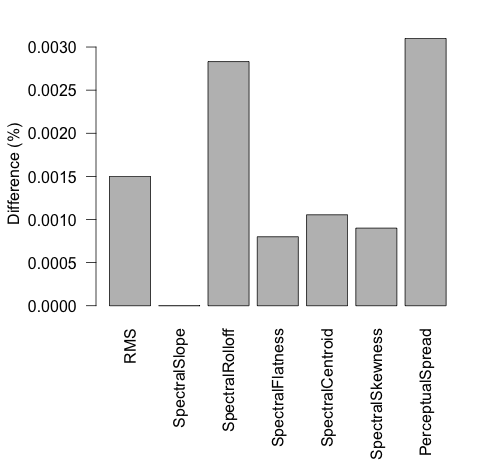
\includegraphics[width=70mm]{YAAFEvsMeyda.png}
\caption{Percentage Differences between YAAFE and Meyda}
\label{fig:error}
\end{figure}

\subsubsection{Results}
In \cref{fig:rolloff,fig:spread,fig:error}, we include plots demonstrating comparisons between the output of several feature extractors in Meyda and YAAFE. These, among others, were used to determine the validity (``sanity-check'') of Meyda's results. In particular, they were applied to a recording of pure white noise (in 150 consecutive buffers), which is by definition bound to produce certain logically inferrable values, even when the analysed buffers are not exactly the same. Therefore the values do not match exactly, but rest in the same ranges. The maximum percentage difference between Yaafe and Meyda results was 0.003\%(on features where we could calculate\footnote{The percentage differences were calculated by taking the absolute value of the individual differences, divided by the feature's output range} the difference), as shown in Figure \ref{fig:error}. It is necessary to note that we are still in the process of optimizing and modifying certain algorithms, e.g. the MFCC implementation.

The `online' extraction paradigm within which Meyda works is reponsible for the slight error in comparison to YAAFE, which works on non-realtime audio. The discrepancy in our testing results is explained by the different start-points of buffers between YAAFE and Meyda. Issues with the `phasing' of buffers in relation to the time domain samples of the audio result in miniscule differences in the numerical results. Our testing was intended to show that our feature extraction algorithms produce `sane' results, as Meyda is not intended to precisely match YAAFE. When we start providing parameterisable extractors there will be greater discrepancies between existing libraries as users start to tailor audio features to meet their use case requirements.

\subsection{Benchmarking}
Assessing the performance of Meyda was necessary to determine that the feature extractors could run comfortably in real-time, and therefore were appropriate for the set of applications that audio feature extraction is widely used in. Despite the fact that there are no comparable implementations of feature extraction libraries specifically targeting the Web Audio API, we ran benchmarking on Meyda to confirm that it was running faster than real-time audio on a relatively standard device. We used benchmark.js to determine running times for each of the extractors separately, then all of them simultaneously.

\subsubsection{Results}

\begin{figure}[ht!]
\centering
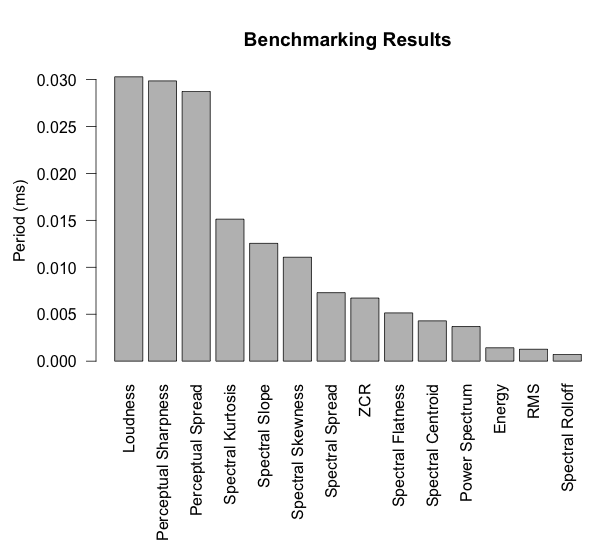
\includegraphics[width=90mm]{512_samples.png}
\caption{Feature extraction times from a buffer of 512 samples}
\end{figure}

Benchmarking indicated that Meyda can comfortably run real-time feature extraction in the browser. Computing all of the features simultaneously on one buffer of 512 samples can be run at 288 operations per second, approximately 3.34 times realtime. Furthermore, specific features such as RMS and spectral rolloff were computed on a much quicker time frame, with RMS calculated approximately 700,000 times per second and spectral rolloff slightly above 1,000,000 times per second.

\subsection{Mobile browsers}

Meyda was tested on two mobile browsers; Firefox 33.0 running on a OnePlus One Android Smartphone (CynanogenMod version 11.0-XNPH38R), and a GeeksPhone Peak (Firefox OS Boot2Gecko 1.3.9.9-prerelease). We were able to simultaneously run all feature extractors except ComplexSpectrum and Loudness on both devices. We aim to make ComplexSpectrum and Loudness both compatible with mobile devices as part of our efforts towards cross-browser compatibility. The fact that these extractors run on mobile devices is very encouraging, as it indicates the potential for applications using feature extraction to be used on smaller, cheaper devices, and broaden the potential uses of this technology.

\section{Future Work}
It is important to bear in mind that the Web Audio API is an emerging specification, and while it is generally quite feature complete, there are certain features that are important for MIR applications and are not in the current version of the specification. When a best practice method of using custom FFT procedures emerges, whether in the Web Audio API or as part of the proposed Web Array Math API, we intend to add extra feature extractors that depend on it, that are currently unfeasible in real-time. Furthermore, plans have emerged within our team to implement an API for higher-level, semantic sound description, using Meyda. This would encompass tools for musical information retrieval, such as beat detection, harmonic functions detection and timbral and temporal segmentation. Additionally, speech recognition based on Meyda's MFCC extraction may be incorporated within this API.

Some features use constants that have been taken from other papers. For example, spectral rolloff is the frequency below which N\% of the energy content is contained, where N is 95\cite{peeters2004large}, 85\cite{jAudio} or 99\cite{mathieu2010yaafe} depending on the source. One way to deal with this would be to add paramaterisation to the feature extractors to allow the user to define the constants that they wish to use, while also providing suitable values.

We intend to improve testing by writing automated unit and integration tests as well as improving our benchmarking suite to more comprehensively test the various combinations of different features at different buffer sizes. There are various tools for this including Travis-CI\cite{travisci} and Jenkins\cite{jenkins}.

Meyda is designed as an open source project, and as such is very much open to contributions from the community in the hopes that we will be left with a sustainable community project. We are particularly interested in contributions related to the optimisation of Meyda, as well as implementations of further feature extractors as listed in \textit{A large set of audio features for sound description (similarity and classification) in the CUIDADO project}~\cite{peeters2004large}.

\section{Conclusions}
Meyda provides a research basis on which to build further technologies for live music information retrieval systems in the browser. As demonstrated, we achieved our aims of meeting the performance levels required for real-time querying of a music information retrieval system, and anticipate that Meyda will be useful for further applications in the web, including but not limited to information retrieval, visualisation, and in-game use in conjunction with the HTML5 canvas element and WebGL. In order to ensure that Meyda provides accurate and reliable results, we have tested it against several popular feature extraction libraries. In praticular, we have performed extensive cross-checking of Meyda against YAAFE, and proved that we meet the quality standards on various types of audio content. We have also used YAAFE in order to construct Meyda's list of features for it to contain the most relevant and useful features. Meyda is still an ongoing project and the Web Audio API specification is under active development, therefore, there is still further work that would be implemented to Meyda in the near future.

\section{Acknowledgments}
The authors would like to thank Dr. Rebecca Fiebrink of Goldsmiths, University of London for providing essential feedback during the development of Meyda. We would also like to thank Dr. Marco Gillies, who along with Rebecca Fiebrink provided feedback on this paper.

\nocite{*}
\bibliographystyle{ieeetr}
\bibliography{sigproc}

\end{document}

\end{document}